The most visible part of any language is its syntax.
Each of us has a different background in terms of programming experience and preferences.
Inadvertently this will introduce some bias in our decision-making, but our distinct preferences
should counteract each other's biases.

Moreover, basing our language on existing languages may be somewhat counterproductive.
On one hand, creating a language that offers some familiarity to experienced programmers is a benefit.
However, following existing conventions defeats the purpose of the project i.e.: creating a language designed around graphs.
This was the mindset we had when setting out to design the syntax of Lattice.

Before getting into the concrete decisions we made, it is important to elaborate on our process, and the questions
we posed to ourselves.

\subsection{Verbosity and Obscurity}\label{subsec:syntax_verbostiy_and_obscurity}
Verbosity and obscurity are two opposing characteristics when designing language.
We could design a language that
relies heavily on English, making it accessible for new developers.
However, incessant verbosity may slow down experienced users when developing code.

Conversely, relying on obscure and arbitrary (but shorter) notations will
steepen the learning curve and may reduce readability.

In general, if we imagine the problem as a curve between verbosity and obscurity, we have fallen closer to
obscure choices with our decisions.
The reason for this is that we had to come up with various, previously
non-existent operators, and built-in functions working on a graph.
We, as a group also have a subjective preference for shorter, more obscure notation, the idea being that
after the initial learning period, its benefits offset the drawbacks.


\subsection{Ambiguity in Ownership and Operators}\label{subsec:syntax_ambigoutiy_in_ownership_and_operators}
The main problem we immediately encountered was ambiguity.
Consider the following questions:

\begin{enumerate}
    \item Can a node be added to two graphs?
    \item Can an edge exist between nodes belonging to different graphs?
\end{enumerate}

Suppose we allow the above behaviour, which we do intend to, as we wish to create a flexible language.
The desired operators are to be detailed later, but one of them is an operator that returns a list of edges belonging to a node.
If we were to apply said operator on a node that belongs to two graphs and has edges within both graphs, the operator would work ambiguously
(figure~\ref{fig:syntax_ambigous}).

\begin{figure}[H]
    \centering
    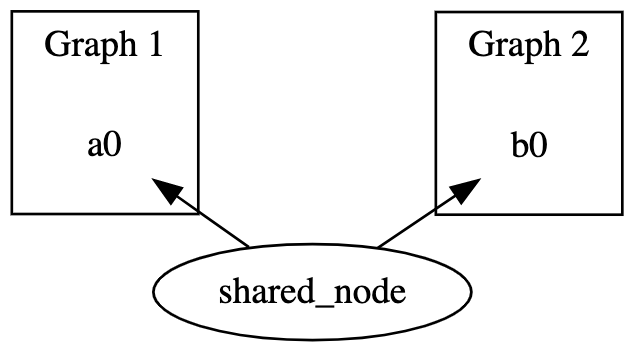
\includegraphics[width=6cm]{figures/syntax_section/syntax_ambigous}
    \caption{An example of a graph displaying a potentially ambigous situation.}
    \label{fig:syntax_ambigous}
\end{figure}


Because it may return any of the following:
\begin{enumerate}
    \item The operator returns the edges defined within graph 1
    \item The operator returns the edges defined within graph 2
    \item The operator returns the edges belonging to both graphs.
\end{enumerate}

Each of these behaviours is equally valid.
Moreover, depending on the context, the user may wish to use any one of them.
The obvious solution is to split the operator into three distinct operators or expand it with a graph parameter.
However, if we consider that this is a single example of the problem, and the actual issue is systematic.
Increasing the operator count or complexity only degrades the readability of the code and introduces the potential for bugs
both when using the language, and when implementing it.

Our proposed solution is therefore to treat graphs as contexts.
Every operation performed inside a context, explicitly belongs to that graph.
Technically, this approach forbids the previously stated questions.
However, we intend to make the graphs nestable.
So while a node cannot belong to two distinct graphs, it may belong to both of them in the context of a parent graph.
Therefore, if we want to get a list of the edges belonging to graph 1, connected to the node, we may perform the
operation in the context of graph 1.
If we want to return all the edges, we may perform it in the context of the parent graph.

\subsection{Assignment and Types}\label{subsec:syntax_assignment_and_types}
Before introducing, the core of Lattice - graphs, it is important to explicitly state basic functionality,
such as variables and assignments.
We have chosen to explicitly state the type of a variable at declaration,
following the form of \lstinline{type var_name = value}.
Listing~\ref{lst:syntax_basic_var_dec} is an example of how variables are declared in Lattice.

We also settled on a set of primitive types we intend to implement, namely:
\begin{itemize}
    \item Integer - (int)
    \item String - (str)
    \item Boolean - (bool)
    \item Float - (float)
\end{itemize}

\begin{lstlisting}[caption={Basic variable declaration.},captionpos=b,label={lst:syntax_basic_var_dec}]
    int a = 1;
    str text = "text";
    bool boolExpr = true;
    float half = 0.5;
\end{lstlisting}



\subsection{Branching}\label{subsec:syntax_branching}
We have decided to implement the simplest form of branching, a simple if-else block.
While additional branching options are nice to have, such as else-if or switch statements, their
expressive power is the as same if-else.

The syntax will be C-like as shown in listing~\ref{lst:syntax_basic_if_else}
\begin{lstlisting}[caption={Simple branching example.},captionpos=b,label={lst:syntax_basic_if_else}]
    bool foo = true;
    if(foo) {
        print "foo"
    }
    else {
        print "bar"
    }
\end{lstlisting}

\subsection{Graphs}\label{subsec:syntax_graphs}
Graphs are the concept, around which the whole language is built around.
Therefore, the definition of graphs
must be simple and concise.
The notation must also allow the usage of contexts.
Ultimately we ended up with a syntactic solution we believe is simple, and easy to read.
Below is an excerpt for
defining a graph with two nodes.

\begin{lstlisting}[caption={Graph declaration.}, captionpos=b, label={lst:syntax_basic_graph_definition}]
    graph g1 {
        ref int a = 5;
        ref str b = "foo";
    }
\end{lstlisting}

\begin{figure}[H]
    \centering
    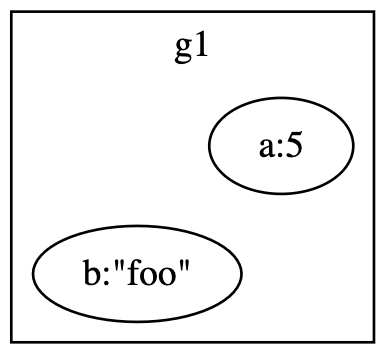
\includegraphics[width=6cm]{figures/syntax_section/syntax_simple_graph}
    \caption{A simple graph generated by~\ref{lst:syntax_basic_graph_definition}}
    \label{fig:syntax_basic_graph}
\end{figure}

Listing~\ref{lst:syntax_basic_graph_definition} generates the graph shown on figure~\ref{fig:syntax_basic_graph}

The graph keyword, when binding the graph may seem unnecessary.
However, a potential extension we have considered was inheritance.
So in the future, one may define a specific type of graph.
E.g. Tree or LinkedList, which conceptually are just restricted graphs.

The context of graphs may be reopened as well.
So the snippet shown on listing~\ref{lst:syntax_basic_graph_definition}
may be extended with a third node (listing~\ref{lst:syntax_basic_graph_defintion_extended})
even after the declaration of the node - generating figure~\ref{fig:syntax_basic_graph_extended}

\begin{lstlisting}[caption={Extending a graph.},captionpos=b,label={lst:syntax_basic_graph_defintion_extended}]
    graph g1 {
        ref int a = 5;
        ref str b = "foo";
    }
    print "outside of the g1 context";
    g1 {
        ref bool c = false;
    }
\end{lstlisting}

\begin{figure}[H]
    \centering
    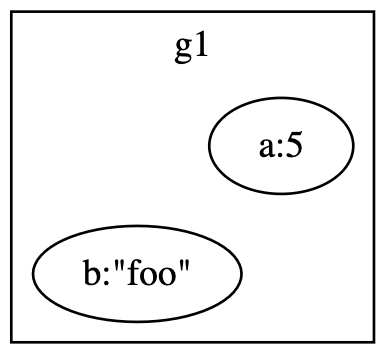
\includegraphics[width=6cm]{figures/syntax_section/syntax_simple_graph}
    \caption{A graph extended by reopening the context, generated by listing~\ref{lst:syntax_basic_graph_defintion_extended}}
    \label{fig:syntax_basic_graph_extended}
\end{figure}

To create sub-graphs, one may open a sub-context inside an existing graph.
The child graph will not implicitly inherit the parent nodes, but they must be explicitly referenced or cloned.
This allows the user to create proper sub-graphs.
Listing~\ref{lst:syntax_basic_subgraph} shows the code for creating such sub-graphs, resulting in figure~\ref{fig:syntax_basic_subgraph}

\begin{lstlisting}[caption={Creating a sub-graph g2 in the context of g1},captionpos=b, label={lst:syntax_basic_subgraph}]
    graph g1 {
        ref int a = 5;
        ref str b = "foo";

        g2 {
            ref a;
        }
    }
\end{lstlisting}
\begin{figure}[H]
    \centering
    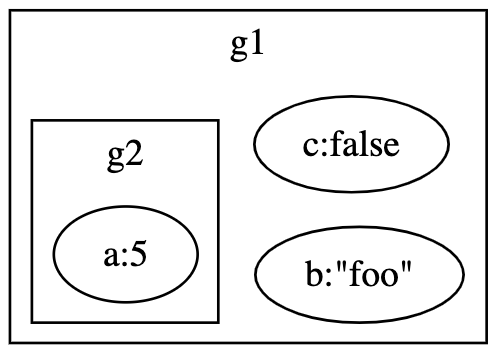
\includegraphics[width=6cm]{figures/syntax_section/syntax_basic_subgraph}
    \caption{A graph extended by reopening the context, generated by~\ref{lst:syntax_basic_subgraph}.}
    \label{fig:syntax_basic_subgraph}
\end{figure}

\subsection{Nodes}\label{subsec:syntax_nodes}
Similar to graphs, nodes ought to be first-class citizens in Lattice.
Initially, we played around with the
idea of having every declared variable act as implicit nodes in the graph.
However, when writing example programs it quickly became a nuisance.
Any program with any degree of complexity will inevitably use \("\)helper\("\) variables.
These variables may be simple things such as loop iterators, or the result of boolean expressions.

Therefore, variables intended to be used as nodes will have to be prefixed either by the ref or the clone keyword.

The keyword naming is self-explanatory.
Ref introduces the node in the graph by its reference, such that if
the node is changed in a different context, its value will change in every graph.
Contrary to that, a cloned node
will be copied over to the graph with its current value.

Listing~\ref{lst:syntax_ref_clone_difference_node} and figure~\ref{fig:syntax_ref_vs_clone} show the difference between ref and clone.

\begin{lstlisting}[caption={Example code, showcasing the difference between ref and clone.},captionpos=b,label={lst:syntax_ref_clone_difference_node}]
    int a = 5;
    int b = 6;

    graph g1 {
        ref a;
        clone b;
    }
    a = 10;
    b = 12;
\end{lstlisting}
\begin{figure}[H]
    \centering
    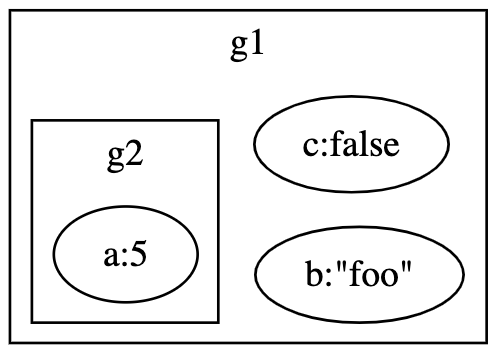
\includegraphics[width=6cm]{figures/syntax_section/syntax_basic_subgraph}
    \caption{A graph extended by reopening the context, generated by listing~\ref{lst:syntax_ref_clone_difference_node}.}
    \label{fig:syntax_ref_vs_clone}
\end{figure}

These keywords may also be applied to graphs when sub-graphing behaviour is required.
Otherwise, the difference in the behaviour of ref and clone is the same.

\begin{lstlisting}[caption={Ref and clone with graphs.},captionpos=b, label={lst:syntax_ref_clone_difference_graph}]

    graph g1 {
        ref int a = 5;
    }
    graph g2 {
        ref int b = 6;
    }
    graph g1ug2 {
        ref g1;
        clone g2;
    }
    g1 {
        ref int a = 10;
    }
    g2 {
        ref int b = 12;
    }
}
\end{lstlisting}
\begin{figure}[H]
    \centering
    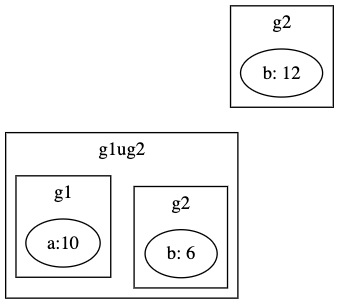
\includegraphics[width=6cm]{figures/syntax_section/syntax_ref_vs_clone_graphs}
    \caption{A graph extended by reopening the context, generated by listing~\ref{lst:syntax_ref_clone_difference_graph}.}
    \label{fig:syntax_ref_vs_clone_with_graphs}
\end{figure}

An interesting discovery we made during the development of mock code, it was much easier to unambiguous code
when the nodes were treated as immutable.
So listing~\ref{lst:syntax_immutability_valid} is a valid Lattice code, while listing~\ref{lst:syntax_immutability_invalid} is not.

\begin{lstlisting}[caption={Valid destruction and recreation of nodes.},captionpos=b,label={lst:syntax_immutability_valid}]
    graph g1 {
        ref int a = 5;
    }
    g1 {
        ref int a = 6;
    }
\end{lstlisting}

\begin{lstlisting}[caption={Code violating the immutability of nodes.},captionpos=b,label={lst:syntax_immutability_invalid}]
    graph g1 {
        ref int a = 5;
    }
    g1 {
        a = 6;
    }
\end{lstlisting}


\subsection{Operators}\label{subsec:syntax_operators}
As mentioned before, we do introduce some obscure notation in our design.
The reasoning is that we want to support operations that are generally either not supported in other languages
or only supported via external libraries that are dependent on the language's own syntax.

While we are not going to change the operator for adding two integers together (int1 + int2).
We are going to create our own arbitrary notation for graph operations since it is a new territory.

For example, if we were to build an edge between two nodes,
Lattice provides the following built-in operators to do so:

\begin{itemize}
    \item \lstinline{node1 <-"label1",5-> node2}
    \item \lstinline{node1 |-"label2",0.5-> node2}
\end{itemize}

Which will generate the graph shown on figure~\ref{fig:relation_basic_operator}
\begin{figure}[H]
    \centering
    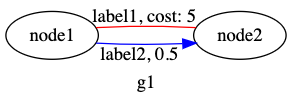
\includegraphics[width=6cm]{figures/syntax_section/syntax_rel_basic}
    \caption{Example graph showcasing various edge operators.}
    \label{fig:relation_basic_operator}
\end{figure}


The first operator creates an undirected edge between node1 and node2, with the label: label1 and a cost of 5.
The second operator creates a directed edge between node1 and node2 where node1 is the predecessor and node2 is the successor.
The labelling and cost behaviour are the same.

In an ideal world, the label and cost parameters would be optional.
However, it is one the restrictions we made to reduce the scope of the project.

We also want to allow programmatic graph traversal.
The easiest way to achieve it is to introduce query operators, which may be used to move along the graph.

\begin{itemize}
    \item \lstinline{node1->?} returns all the directed edges where node1 is the predecessor.
    \item \lstinline{?->node1} returns all the directed edges where node1 is the successor.
    \item \lstinline{node1-|?} returns every undirected edge connected to node1.
    \item \lstinline{rel1?} returns the successor node of rel1.
    \item \lstinline{?rel1} returns the predecessor node of rel1.
    \item \lstinline{?rel2?} returns a pair of nodes, assuming that rel1 is an undirected edge.
\end{itemize}

If the above operators were applied on the graph shown on figure~\ref{fig:syntax_query_operators_example_out}.
The following would be returned:

\begin{itemize}
    \item \lstinline{node1->?} returns node2.
    \item \lstinline{?->node1} returns node3.
    \item \lstinline{node1-|?} returns node2 and node4.
    \item \lstinline{rel1?} returns node2.
    \item \lstinline{?rel1} returns node1.
    \item \lstinline{?rel2?} returns node1 and node4.
\end{itemize}

\begin{figure}[H]
    \centering
    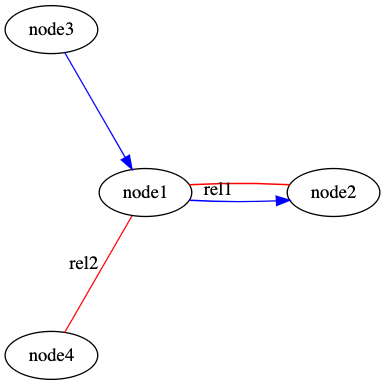
\includegraphics[width=6cm]{figures/syntax_section/syntax_query_operators}
    \caption{Example graph to show the usage of query operators.}
    \label{fig:syntax_query_operators_example_out}
\end{figure}

Besides the graph-specific operators, we include a suite of well-known basic operators.
Below is a categorized list of the operators we intend to implement:


\textbf{Boolean operators}
\begin{itemize}
    \item \lstinline{&&} - boolean \emph{and} operator.
    \item \lstinline{||} - boolean \emph{or} operator.
    \item \lstinline{!} - boolean \emph{negate} operator.
    \item \lstinline{==} - boolean \emph{equality} operator.
    \item \lstinline{!=} - boolean \emph{inequality} operator.

\end{itemize}

\textbf{Numeric operators}
\begin{itemize}
    \item \lstinline{+} - \emph{addition}.
    \item \lstinline{-} - \emph{subtraction}.
    \item \lstinline{*} - \emph{multiplication}.
    \item \lstinline{/} - \emph{division}.
    \item \lstinline{%} - \emph{remainder}.
    \item \lstinline{<} - \emph{larger than}.
\end{itemize}

There are some well-known operators left out, such as \lstinline{<=} or \lstinline{>}.
Simply because while it is arduous to work around them, it is still possible to do so.
For example  \lstinline{int1 <= int2} may be expressed with:  \lstinline{int1 < int2 || int1==int2}.

\subsection{Edges}\label{subsec:syntax_edges}
The final, essential component for a language for graphs are edges.
In the previous section, their operators have been introduced.
They do, however, have to exist as standalone objects as well.
If they only exist within the operations, the power of the language is rather
limited.

Therefore, the above-mentioned operation node1 \lstinline{<-"label1",5-> node2}, returns a relationship object (a common, shared
type for directed and undirected edges).

So, the following would be valid code in Lattice: \lstinline{rel r = node1 <-"label1",5-> node2.}

Then, the developer may apply any of the relationship operations on r.

\subsection{Functions}\label{subsec:syntax_functions}
Functions were one of those well-known features that needed to be included in Lattice.
Having reusable blocks of code made developing example code significantly easier.

In line with our implementation of \("\)if-else\("\) and \("\)while\("\) we have chosen to implement functions in a C-like manner.
They follow the basic structure of:

\lstinline|return_type function_name (arg_type arg_name) {statements; return return_value;}|

An example is shown in listing~\ref{lst:syntax_fmap_basic}

\subsection{Iteration and Enumeration}\label{subsec:syntax_iteration-and-enumeration}
Iteration, in the classical sense, is a simple, and well-explored problem.
We have chosen to only include while loops (listing~\ref{lst:syntax_syntax_while_basic})
in Lattice, as its expressive power, is equivalent to any other constructs, such as for, or foreach.

\begin{lstlisting}[caption={Simple while loop.},captionpos=b,label={lst:syntax_syntax_while_basic}]
    int iterator = 0;
    int max = 5;
    while(iterator < max) {
        print iterator;
    }
\end{lstlisting}


The main question, however, is, how does one enumerate a graph?
Currently, there is no commonly accepted approach
for such operations.

Building a deterministic approach would be relatively easy.
We could, for example, apply the operations on the nodes in which
they were added.

However, we believe that the nature of the answers point to the fact that traditional approaches are insufficient for graph
enumeration.

Therefore, we have decided to try a functional approach.
Haskell's fmap fits our needs precisely.
It is a function that takes a function, and a custom data type as input, and applies the function to each member of
the entity.
The underlying implementation does not concern the user, nor is it apparent when it is used.

For example, in listing~\ref{lst:syntax_fmap_basic} we apply the function double to g1, and return a cloned instance
in the form of g2 (figure~\ref{fig:syntax_fmap_basic})

\begin{lstlisting}[caption={Simple fmap application on a graph.},captionpos=b,label={lst:syntax_fmap_basic}]
    graph g1 {
        ref int a = 5;
        ref int b = 6;
        ref int c = 7;

       a |-"ab",0-> b;
       b |-"bc",0-> c;
       c |-"ca",0-> a;
    }
    graph g2 = fmap double g1;

    int double(int node) {
        return node*2;
    }
\end{lstlisting}

\begin{figure}[H]
    \centering
    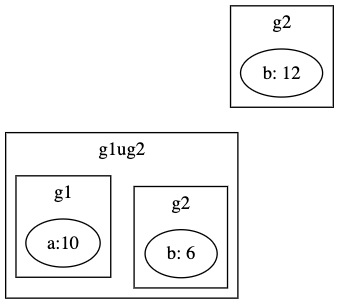
\includegraphics[width=6cm]{figures/syntax_section/syntax_ref_vs_clone_graphs}
    \caption{An application of fmap, where g2 is a clone of g1, with the double function applied. Generated by listing~\ref{lst:syntax_fmap_basic}.}
    \label{fig:syntax_fmap_basic}
\end{figure}


\subsection{Polymorphic Implications}\label{subsec:syntax_polymorphic_implications}
A notable omission from the previous sections was type behaviour.
If we were to consider that graphs do not have a single
type of node they accept like other strongly typed languages, such as C\# (\lstinline[language=C#]{List<int> intList = new List<int>();}),
and that fmap may be applied to any graphs, the code shown on~\ref{lst:syntax_invalid_fmap} is syntactically valid Lattice code.

\begin{lstlisting}[caption={Fmap applied on a graph that contains non-numeric values.},captionpos=b,label={lst:syntax_invalid_fmap}]
graph g {
    ref string a = "a";
    ref bool b = true;
    ref int c = 1;
}
graph g2 = fmap (+1) g;
\end{lstlisting}


This is the reason why we decided to have the nodes strongly typed.
With strongly typed nodes we may perform compile time type check, therefore while the syntax is valid,
it would be semantically invalid, and would result in a compiler error.


\subsection{Showcase: K-Sized Binary Tree}\label{subsec:syntax_showcase_k_sized_binary_tree}
Listing~\ref{lst:syntax_k_sized_tree} illustrates a potential program that may be written in Lattice.
It generates a binary tree of height K.
It does so by duplicating the previous instance of the tree, and connecting them by a new common root.

\begin{lstlisting}[caption={Lattice code generating a balanced binary tree of height K.},captionpos=b,label={lst:syntax_k_sized_tree}]
    int k = 5;
    int iterator = 0;
    str nodeVal = "node";
    str leftRoot;
    str rightRoot;


    graph left {}
    graph right {}
    graph bTree {
    }
    while(iterator < k) {
        if(iterator == 0) {
            bTree {
                clone nodeVal;
                str newRoot = nodeVal;
            }
        }
        else {
            bTree {
                clone left;
                clone right;

                newRoot |-"left",0-> leftRoot;
                newRoot |-"right",0-> rightRoot;

            }
        }
        left = clone bTree;
        right = clone bTree;
        left {
            str leftRoot = newRoot;
        }
        right {
            str rightRoot = newRoot;
        }
        iterator = iterator + 1;
    }
\end{lstlisting}